\documentclass{standalone}
\usepackage{graphicx}	
\usepackage{amssymb, amsmath, amsthm}
\usepackage{color}

\usepackage{tikz}
\usetikzlibrary{intersections, backgrounds}

\definecolor{light}{RGB}{220, 188, 188}
\definecolor{mid}{RGB}{185, 124, 124}
\definecolor{dark}{RGB}{143, 39, 39}
\definecolor{highlight}{RGB}{180, 31, 180}
\definecolor{gray10}{gray}{0.1}
\definecolor{gray20}{gray}{0.2}
\definecolor{gray30}{gray}{0.3}
\definecolor{gray40}{gray}{0.4}
\definecolor{gray60}{gray}{0.6}
\definecolor{gray70}{gray}{0.7}
\definecolor{gray80}{gray}{0.8}
\definecolor{gray90}{gray}{0.9}
\definecolor{gray60}{gray}{0.95}

\begin{document}

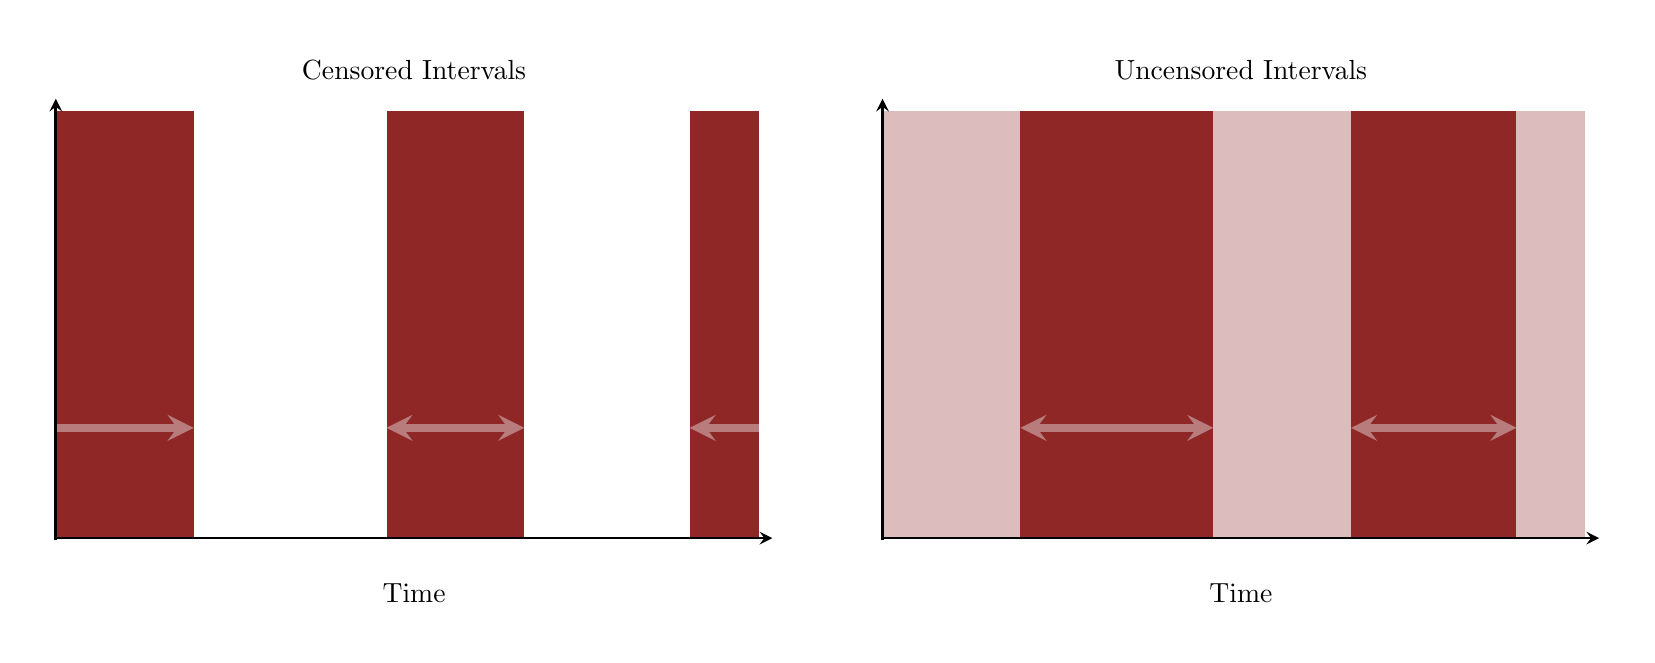
\begin{tikzpicture}[scale=0.35]
  \begin{scope}[shift={(0, 0)}]
    \draw[white] (-14, -11.5) rectangle (14, 10.5);
    
    \node at (0, 9) { Censored Intervals };
    
    \fill[dark] (-13, -8) rectangle (-8, 7.5);
    \draw[->, >=stealth, line width=3, mid] (-13, -4) -- (-8, -4);
    
    \fill[dark] (-1, -8) rectangle (4, 7.5);
    \draw[<->, >=stealth, line width=3, mid] (-1, -4) -- (4, -4);
    
    \fill[dark] (10, -8) rectangle (12.5, 7.5);
    \draw[<-, >=stealth, line width=3, mid] (10, -4) -- (12.5, -4);
  
    \draw [->, >=stealth, line width=1] (-13, -8) -- +(26, 0);
    \draw [->, >=stealth, line width=1] (-13, -8.058) -- +(0, 16);
    \node[] at (0, -10) { Time };
  \end{scope}
  
  \begin{scope}[shift={(30, 0)}]
    \draw[white] (-14, -11.5) rectangle (14, 10.5);
    
    \node at (0, 9) { Uncensored Intervals };
    
    \fill[light] (-13, -8) rectangle (-8, 7.5);
    
    \fill[dark] (-8, -8) rectangle (-1, 7.5);
    \draw[<->, >=stealth, line width=3, mid] (-8, -4) -- (-1, -4);
    
    \fill[light] (-1, -8) rectangle (4, 7.5);
    
    \fill[dark] (4, -8) rectangle (10, 7.5);
    \draw[<->, >=stealth, line width=3, mid] (4, -4) -- (10, -4);
    
    \fill[light] (10, -8) rectangle (12.5, 7.5);
  
    \draw [->, >=stealth, line width=1] (-13, -8) -- +(26, 0);
    \draw [->, >=stealth, line width=1] (-13, -8.058) -- +(0, 16);
    \node[] at (0, -10) { Time };
  \end{scope}
   
\end{tikzpicture}

\end{document}  